\chapter{Introduction}
\label{chapter:Introduction}

\chapabstract{``In the beginning, there were types.''}

Our story begins with the (over-ambitious, in hindsight) ravings of one of the world's most well-renowned mathematicians, David Hilbert. 
Unhappy with the numerous paradoxes and inconsistencies of mathematics at the end of the 19th century, Hilbert would postulate the existence and advocate the formulation of a finite set of axiomatic rules, which, when put together, would give rise to the most well-behaved system known to [wo]mankind, capable of acting as a universal meta-theory for all mathematics, in the process absolving all mathematicians of their sins.
The idea was of course appealing and gained traction, not the least due to Hilbert's influence over the field (and his will to exercise it).
As with all ideas that generate traction, however, it was not long before a cultural counter-movement would develop.
Intuitionism, with Luitzen Egbertus Jan Brouwer as its forefather, would challenge Hilbert's program by questioning the objective validity of (any) mathematical logic.
What it would claim, instead, is that mathematics is but a subjective process of construction that abides by some rules of inference, which, internally consistent as they may be, hold no reflection of deeper truth or meaning.
In practice, intuitionists would reject the law of the excluded middle (an essential tool for Hilbert's school of formalists) and argue that for a proof to be considered valid, it has to provide concrete instructions for the construction of the object it claims to prove.
The dispute went on for a couple of decades, its flame carried on by the respective students of the two rivals.
Logic, intrigue, conflict, fame, no \LaTeX{} errors...  these truly were the years to be an active mathematician.
Eventually, in a critical moment of clarity and inspiration, and tired by the ongoing drama, Kurt G\"odel, with his famous incompleteness theorem, would declare Hilbert's program unattainable, thus putting a violent end to the line of formalist heathens, and paving the way for the true revolution that was to come.
This is in reference, of course, to the biggest discovery of the last century\footnote{In proof theory, at least.}, made independently (using wildly different words every time) by various mathematicians and logicians spanning different timelines.
Put plainly, what is now known as the Curry-Howard correspondence establishes a syntactic equivalence between deductive systems in intuitionistic brands of logic and corresponding computational systems, called $\lambda$-calculi.
Put even more plainly, it suggests that valid proofs in such logics constitute in fact compilable code for functional progams, bridging in essence the seemingly disparate fields of mathematical logic and computer science.
The repercussions of this discovery were enormous, and are more tangible today than ever before; type systems comprised of higher-order $\lambda$-calculi and their logics provide the theoretical foundations for modern programming languages and proof assistants (this last fact is both important and interesting, but won't concern us much presently).

In a more niche (but equally beautiful) fragment of the academic world, and in parallel to the above developments, applied logicians and formally inclined linguists have been demonstrating a stunning perserverance in their self-imposed quest of modeling natural language syntax and semantics, making do only with the vocabulary provided by formal logics.
The modern incarnation of this noble endeavour is due to Jim Lambek, who was the first to point out that the grammaticality of a natural language utterance can be equated to provability in a certain logic (or type inhabitation, if one is to borrow the terminology of constructive type theories), if the grammar (a collection of empirical linguistic rules) were to be treated as a substructural logic (a collection of formal mathematical rules).
Funnily enough, the kind of logics Lambek would employ for his purposes would be exactly those at the interesection of intuitionistic and linear logic, the latter only made formally explicit in a breakthrough paper by Jean-Yves Girard almost three decades later.
By that time, Richard Montague had already come up with the fantastically novel idea of seeing no distinction between formal and natural languages, single-handedly birthing and popularizing the field of formal semantics (which would chiefly invole semantic computations using $\lambda$-calculus notation), thus fulfilling Gottlob Frege's long-prophesized principle of compositionality, which would once and for all put the Chomskian tradition to rest\footnote{In some corners of the world, this part of the prophecy is yet to transpire.}, ushering linguistics into a new era.
With the benefit of posterity, it would be tempting for us to act smart and exclaim that Lambek and Montague's ideas were remarkably aligned. 
In reality, it took another couple of decades for someone to notice.
The credit is due to Johan van Benthem, who basically pointed out that Lambek's calculi make for the perfect syntactic machinery for Montague's program, seeing as they admit the Curry-Howard correspondence, and are therefore able to drive semantic composition virtually for free (in fact one could go as far as to say that they are the only kind of machinery that can accomplish such a feat without being riddled with ad-hoc transformations).
This revelation, combined with the contemporary bloom of substructural logics, was the spark that ignited a renewed interest in Lambek's work.
The culmination point for this interest was typelogical grammars (or categorial type logics): families of closely related type theories extending the original calculi of Lambek with unary operators lent from modal logic, intended to implement a stricter but more linguistically faithful modeling of the composition of natural language form and meaning.

In this chapter, we will isolate some key concepts from this frantic timeline and expound a bit on their details.
No novel contributions are to be found here; the intention is to establish some common grounds before we get to proceed. 
If confident in your knowledge of the subject matter, \texttt{goto} Chapter~\ref{chapter:chapter_2}.

\subsubsection*{Key References}

\newpage

\section{The Simple Theory of Types}

Simple type theory is the computational formalization of intuitionistic logic. 
It is in essence an adornment of the rules of intuitionistic logic with the computational manipulations they dictate upon mathematical terms.
Dually, it provides a decision procedure that allows one to infer the type of a given program by inspecting the operations that led up to its construction.
It is a staple of almost folkloric standing for computer scientists across the globe, tracing its origins to the seminal works of Russel and Church~\cite{russel1908,church1940}.
The adjective ``simple'' is not intended as either a diminutive nor a condescending remark pertaining to the difficulty of the subject matter, but rather to distinguish it from the broader class of intuitionistic type theories, which attempt to systematize the notions of quantification (universal and existential), stratification of propositional hierarchies, and more recently equivalence (neither of which we will concern ourselves with).

Our presentation will begin with intuitionistic logic. 
Once that is done, we will give a brief account of the the Curry-Howard correspondence, which shall allow us to give a computational account of the logic, that being the simply typed $\lambda$-calculus.

\subsection{Intuitionistic Logic}
\label{subsection:intuitionistic_logic}
Intuitionistic logic is due to Arend Heyting~\cite{heyting1930}, who was the first to formalize Bouwer's intuitionism.
It is a restricted version of classical logic, where the laws of the excluded middle (\textit{tertium non datur}) and the elimination of the double negation no longer hold universally.
The first states that one must choose between a proposition $\prop{A}$ and its negation $\neg \prop{A}$ ($p \wedge \neg \prop{A}$), whereas the second that a double negation is equivalent to an identity ($\neg \neg \prop{A} \equiv \prop{A}$).
The absence of these two laws implies that several theorems of classical logic are no longer derivable in intuitionistic logic, meaning that the logic is weaker in terms of expressivity.
On the bright side, it has the pleasant effect that proofs of intuitionistic logic are constructive, i.e. they explicitly demonstrate the formation of a concrete instance of whatever proposition they claim to be proving.

Focusing on the disjunction-free fragment of the logic, we have a tiny recursive language that allows us to define the various shapes of logical \textit{propositions} (or \textit{formulas}).%
\footnote{The full logic also includes disjunctive formulas, but we will skip them from this presentation as they are of little interest to us. For brevity, we will from now on use intuitionistic logic to refer to its disjunction-free fragment.}
Given some finite set of \textit{propositional constants} (or \textit{atomic formulas}) \propcon{}, and \prop{A}, \prop{B}, \prop{C} arbitrary well-formed propositions, the language of propositions in Backus-Naur form is inductively defined as 
\begin{equation}
\prop{A}, \prop{B}, \prop{C} ::= p \ | \ \prop{A} \to \prop{B} \ | \ \prop{A} \times \prop{B} 
\tag{$\IL_{\to, \times}$}
\label{grammar:IL}
\end{equation}
where $p \in \propcon{}$.
Propositions are therefore closed under the two binary \textit{logical connectives} $\to$ and $\times$; we call the first an \textit{implication}, and the second a \textit{conjunction}. 
A \textit{complex} proposition is any proposition that is not a member of \propcon{}, and its \textit{primary} (or main) connective is the last logical connective used when writing it down according to the grammar~\ref{grammar:IL}.

Besides propositions, we have \textit{structures}. 
Structures are built from propositions with the aid of a single binary operation, the notation and properties of which can vary between different presentations of the logic.
In our case, we will indicate valid structures with greek uppercase letters $\Gamma$, $\Delta, \Theta$, and define structures inductively as 
\[
	\Gamma, \Delta, \Theta ::= 1 \ | \ \prop{A} \ | \ \Gamma, \Delta
\]
In other words, structures are an inductive set closed under the operator $\_,\_$ which satisfies associativity and is equipped with an identity element $1$ (the \textit{empty} structure), i.e. a monoid.
A perhaps more down-to-earth way of looking at a structure is as a \textit{list} or \textit{sequence} of propositions.

Given propositions and structures, we can next define \textit{judgements}, statements of the form
$\Gamma \vdash \prop{A}$.
We read such a statement as a suggestion that from \textit{assumptions} $\Gamma$ (i.e. a structure of \textit{hypotheses}) one can derive a proposition \smallprop{A}.
Formulas occurring within $\Gamma$ are said to occur in \textit{antecedent} position, whereas \prop{A} is in \textit{succedent} position.

A \textit{rule} is a two-line statement separated by a horizontal line.
Above the line, we have a (possibly empty) sequence of judgements, which we call the \textit{premises} of the rule.
Below the line, we have a single judgement, which we call the rule's \textit{conclusion}.
The rule can be thought of as a formal guarantee that if all of its premises are deliverable, then so is the conclusion.
Each rule has an identifying name, written directly to the right of the horizontal line.

Rules may be split in two conceptual categories.
\textit{Logical} rules, on the one hand, provide instructions for eliminating and introducing logical connectives.
Figure~\ref{subfigure:intuitionistic_logic_rules:logical} presents the logical rules of intuitionistic logic.
The first rule, the axiom of identity $Ax$, contains no premises and asserts the reflexivity of the provability operator $\vdash$. 
It states that from a proposition \prop{A} one can infer that very proposition (duh!).
The remaining logical rules come in pairs, one per logical connective.
The elimination of the implication (or modus ponens) states that, given a proof of a proposition $\prop A \to \prop B$ from assumptions $\Gamma$ and a proof of proposition \prop{A} from assumptions $\Delta$, one can join the two to derive a proposition \prop{B}.
Dually, the introduction of the implication (or \textit{deduction theorem}) states that from a proof of a proposition \prop{B} given assumptions $\Gamma, \prop{A}$, one can use $\Gamma$ alone to derive an implicational proposition $\prop A \to \prop B$.
In a similar manner, the elimination of the conjunction $\times E $ states that, given a proof of a proposition $\prop A \times \prop B$ from assumptions $\Gamma$, and a proof that the triplet $\Delta, \prop A, \prop B$ allows us to derive a proposition $\prop C$, one could well use $\Gamma$ together with $\Delta$ to derive $\prop C$ directly.
And dually again, the introduction of the conjunction $\times I$ permits us to join two unrelated proofs, one of $\prop A$ from $\Gamma$ and one of $\prop B$ from $\Delta$ into a single proof, that of their product $\prop A \times \prop B$, from $\Gamma$ joined with $\Delta$.

\textit{Structural} rules, on the other hand, allow us to manipulate structures; they are presented in Figure~\ref{subfigure:intuitionistic_logic_rules:structural}.
Structural rules have a two-fold role.
First, they explicate an extra propery of our structure binding operator, namely commutativity.
One could also make do with an implicit $\Exchange{}$ rule by treating structures as \textit{multisets} rather than lists -- having it explicit, however, will keep us conscious of its presence and strengthen our emotional bond to it, in turn making us really notice its absence when it will no longer be there (it also keeps the presentation tidier).
Second, they give an account of the status of propositions as reusable resources.
The $\Weakening{}$ rule states that if we were able to derive a proposition \prop{B} from some assumptions $\Gamma$, we will also be able to do so if the assumptions were to contain some arbitrary extra proposition \prop{A}.
Conversely, the $\Contraction{}$ rule states that if we needed some assumption structure containing two instances of a proposition \prop{A} to derive a proposition \prop{B}, we could also make do with just one instance of it, discarding the other without remorse.

A \textit{proof}, finally, is a heterogeneous variadic tree.
At its root, it has a judgement, guaranteed to be derivable (provided we did not mess up somewhere).
Its branches are themselves proofs, fused together by a rule -- the number of premises being the local tree's arity.
At its leaves, it has identity axioms -- the smallest kind of proof.

\begin{figure}
	\centering
	\begin{subfigure}{1\textwidth}
		\centering
		\begin{tabularx}{0.7\textwidth}{@{}C@{\qquad}C@{}}
		\multicolumn{2}{@{}c@{}}{$\infer[Ax]{\prop A \vdash \prop A}{}$}\\[1em]
		$\infer[\to E]{\Gamma, \Delta \vdash \prop B}{\Gamma \vdash \prop A \to \prop B & \Delta \vdash \prop B}$ 
		& 
		$\infer[\to I]{\Gamma \vdash \prop A \to \prop B}{\Gamma, \prop A \vdash \prop B}$\\[1em]
		$\infer[\times E]{\Gamma,\Delta \vdash \prop C}{\Gamma \vdash \prop A \times \prop B & \Delta, \prop A , \prop B \vdash \prop C}$ 
		&
		$\infer[\times I]{\Gamma, \Delta \vdash \prop A \times \prop B}{\Gamma \vdash \prop A & \Delta \vdash \prop B}$
		\end{tabularx}
		\caption{Logical rules.}
		\label{subfigure:intuitionistic_logic_rules:logical}
	\end{subfigure}\\[2em]
	\begin{subfigure}{1\textwidth}
		\centering
		\begin{tabularx}{0.7\textwidth}{@{}C@{\qquad}C@{}}
		\multicolumn{2}{@{}c@{}}{$\infer[\Exchange{}]{\Delta, \Gamma \vdash \prop A}{\Gamma, \Delta \vdash \prop A}$}\\[1em]
		$\infer[\Weakening{}]{\Gamma, \prop A \vdash \prop B}{\Gamma \vdash \prop B} $ 
		&
		$\infer[\Contraction{}]{\Gamma, \prop A \vdash \prop B}{\Gamma, \prop A, \prop A \vdash \prop B}$
		\end{tabularx}
		\caption{Structural rules.}
		\label{subfigure:intuitionistic_logic_rules:structural}
	\end{subfigure}
	\caption{Intuitionistic Logic $\IL_{\to,\times}$.}
	\label{figure:intuitioistic_logic_rules}
\end{figure}

\subsubsection{Proof Equivalences}
The same judgement may be provable in more than one ways.
The difference between two proofs of the same judgement can be substantial, when they indeed describe distinct derivation procedures, or trivial.
Trivial variations come in two kinds: syntactic equivalences (i.e. sequences of rule applications that can safely be rearranged) and redundant detours (i.e. sequences of rule applications that can altogether removed).

The first kind is not particularly noteworthy.
In essence, we say that two proofs are syntactically equivalent if they differ only in the positioning of structural rule applications.
This notion can be formally captured by establishing an equivalence relation between proofs on the basis of commuting conversions.

The second kind is more interesting and slightly more involved.
A proof pattern in which a logical connective is introduced, only to be immediately eliminated, is called a \textit{detour} (or $\beta$ redex).
Detours can be locally resolved via proof rewrites -- the fix-point of performing all applicable resolutions is called \textit{proof normalization} and yields a canonical proof form. 
The strong normalisation property guarantees that a canonical form exists for any proof in the logic, and in fact the choice of available rewrites to apply at each step is irrelevant, as all paths have the same end point~\cite{groote1999strong}.
Figure~\ref{figure:intuitionistic_proof_reduction} presents rewrite instructions for the two detour patterns we may encounter (one per logical connective).
Read bottom-up%
\footnote{In the small-to-big rather than literal sense! If confused: start from the proof leaves and go down.},
the first one suggests that if one were to hypothesize a proposition $\smallprop{A}$, use it within an (arbitrarily deep) proof $s$ together with extra assumptions $\Gamma$ to derive a proposition $\smallprop{B}$, before finally redacting the hypothesis and composing with a proof $t$ that derives $\smallprop{A}$ from assumptions $\Delta$, it would have been smarter (and more concise!) to just plug in $t$ directly when previously hypothesizing $\smallprop{A}$, since then no redaction or composition would have been necessary.
In a similar vein, the second suggests that if one were to derive and merge proofs $s$ and $t$ (of propositions $\smallprop{A}$ and $\smallprop{B}$, respectively), only to eliminate their product against hypothetical instances of $\smallprop{A}$ and $\smallprop{B}$ that were used to derive some $\smallprop{C}$ with extra assumptions $\Theta$ within proof $u$, the proof can be reduced by just plugging $s$ and $t$ in place of the axiom leaves of $u$.
Note the use of horizontal dots at the axiom leaves, denoting simultaneous substitutions of \textit{all} occurrences of redundant hypotheses, and the use of unnamed vertical dots, denoting (invertible) sequences of \Contraction{} and/or \Exchange{} rules.

\begin{figure}
	\begin{subfigure}{1\textwidth}
		\begin{tabularx}{0.95\textwidth}{@{}c@{~}c@{~}c@{}}
		$\infer[\to E]{\Gamma, \Delta \vdash \prop{B}}{
		\infer[\to I]{\Gamma \vdash \prop{A} \to \prop{B}}{
			\infer*[]{\Gamma, \prop{A} \vdash \prop{B}}{
				\infer[]{\Gamma, \prop{A} \dots \vdash \prop{B}}{
						\infer*[s]{}{\dots & \infer[Ax]{\prop{A} \vdash \prop{A}}{}}
					}
				}
			}
			&
			\infer{\Delta \vdash \prop{A}}{
				\infer*[t]{}{}
			}
		}$
		&
		\raisebox{20pt}{$\implies$}
		&
		$ 
		\infer*[]{\Gamma, \Delta \vdash \prop{B}}{
			\infer[]{\Gamma, \Delta \dots \vdash \prop{B}}{
				\infer*[s]{}{
				\dots &
				\infer[]{\Delta \vdash A}{
					\infer*[t]{}{}
				}}
			}
		}
		$\\[2em]
		$
		\infer[\times E]{\Gamma, \Delta, \Theta \vdash \prop{C}}{
			\infer[\times I]{\Gamma, \Delta \vdash \prop{A} \times \prop{B}}{
				\infer[]{\Gamma \vdash \prop{A}}{\infer*[s]{}{}}
				&
				\infer[]{\Delta \vdash \prop{B}}{\infer*[t]{}{}}
			}		
			&
			\infer*[]{\Theta, \prop{A}, \prop{B} \vdash \prop{C}}{
				\infer[]{\Theta, \prop{A}, \prop{B}\dots \vdash \prop{C}}{
					\infer*[u]{}{
						\infer[Ax]{\prop{A} \vdash \prop{A}}{
						}
						&
						\dots
						&
						\infer[Ax]{\prop{B} \vdash \prop{B}}{}
					}
				}
			}
		}
		$
		&
		\raisebox{20pt}{$\implies$}
		&
		$
		\infer*[]{\Gamma, \Delta, \Theta \vdash \prop{C}}{
			\infer[]{\Gamma, \Delta, \Theta \dots \vdash \prop{C}}{
				\infer*[u]{}{
					\infer[]{\Gamma \vdash \prop{A}}{
						\infer*[s]{}{}
					}
					&
					\dots 
					&
					\infer[]{\Delta \vdash \prop{B}}{
						\infer*[t]{}{}
					}
				}
			}
		} 
		$
		\end{tabularx}
		\label{123}
		\caption{123}
	\end{subfigure}
	\caption{Intuitionistic proof reductions.}
	\label{figure:intuitionistic_proof_reduction}
\end{figure}


\subsection{The Curry-Howard Correspondence}
The Curry-Howard correspondence asserts an equivalence between the above presentation of the logic in natural deduction, and a system of computation known as the $\lambda$-calculus.
It was first formulated by Haskell Curry in the 30s before being independently rediscovered by William Alvin Howard and Nicolas Goveert de Bruijn in the 60s~\cite{curry1934functionality,de1983automath,howard1980formulae}.
The entry point for such an approach is to interpret propositions as \textit{types} of a minimal functional programming language (a perhaps more aptly named alternative to the Curry-Howard correspondence is the \textit{propositions-as-types interpretation}).
In that sense, the set of propositional constants \propcon{} becomes the programming language's basic set of \textit{primitive} types (think of them as built-ins).
Implicational formulas $\prop A \to \prop B$ are read as \textit{function} types, and conjunction formulas are read as \textit{tuple} (or cartesian product) types.
From now we will use formulas, propositions and types interchangeably.
Following along the correspondence allows us to selectively speak about individual, named instances of propositions -- we call these \textit{terms}.
The simplest kind of term is a \textit{variable}, corresponding to a hypothesis in the proof tree.
Each logical rule is identified with a programming pattern: the axiom rule is variable \textit{instantiation}, introduction rules are \textit{constructors} of complex types, and elimination rules are their \textit{destructors}.
The question of whether a logical proposition is provable translates to the question of whether the corresponding type is inhabited; i.e. whether an object of such a type can be created -- we will refer to the latter as a \textit{well-formed} term.

Rather than present a grammar of terms and later ground it in the logic, we will instead simply revisit the rules we established just above, now adorning each with a term rewrite instruction -- the result is a tiny yet still elegant and expressive type theory, presented in Figure~\ref{figure:simple_type_theory}.
Given an enumerable set $\mathcal{V}$ of unique names for indexed variables, with elements \term{x_i}, and denoting arbitrary but well-formed terms with \term{s}, \term{t}, \term{u}, we will use $\term{s}: \prop{A}$ (or $\term{s}^{\smallprop{A}}$) to indicate that term \term{s} is of type \prop{A}.
Assumptions $\Gamma$, $\Delta$ will now denote a \textit{typing environment}:
\[
\term x_1 : \prop  A_1 ,~ \term x_2 : \prop A_2 \dots ~ \term x_n : \prop A_n
\]
i.e. rather than a sequence of formulas, we have a sequence of distinct variables, each of a specific type, and a judgement $\Gamma \vdash \term{s} : \prop{B}$ will now denote the derivation of a term \term{s} of type \prop{B} out of such an environment.

\begin{figure}
	\centering
	\begin{tabularx}{0.975\textwidth}{@{}C@{~}C@{}}
		\multicolumn{2}{@{}c@{}}{$\infer[Ax]{\term{x_i} : \prop A \vdash \term{x_i} : \prop A}{}$}\\[2em]
		$\infer[\to E]{\Gamma, \Delta \vdash \term{s~t} : \prop B}{\Gamma \vdash \term{s} : \prop A \to \prop B & \Delta \vdash \term{t} : \prop B}$ 
		& 
		$\infer[\to I]{\Gamma \vdash \term{\lambda x_i.s} : \prop A \to \prop B}{\Gamma, \term{x_i}: \prop A \vdash \term{s}:\prop B}$\\[2em]
		$\infer[\times E]
			{\Gamma,\Delta \vdash
			 \cterm{case \term{s} of (\term{x_i}, \term{x_j}) in \term{t}} 
			 : \prop{C}}
			{\Gamma \vdash \term{s}: \prop A \times \prop B & 
			\Delta, \term{x_i}: \prop A , \term{x_j}: \prop B \vdash \term{t}: \prop{C}}$ 
		&
		$\infer[\times I]
			{\Gamma, \Delta \vdash \cterm{(\term{s}, \term{t})}: \prop{A} \times \prop{B}}
			{\Gamma \vdash \term{s}: \prop{A} & \Delta \vdash \term{t}:\prop{B}}$\\[2em]
		\multicolumn{2}{@{}c@{}}{$\infer[\Exchange{}]{\Delta, \Gamma \vdash \term{s}: \prop{A}}{\Gamma, \Delta \vdash \term{s}: \prop{A}}$}\\[2em]
		$\infer[\Weakening{}]
			{\Gamma, \term{x_i}: \prop{A} \vdash \term{s}: \prop{B}}
			{\Gamma \vdash \term{s}:\prop{B}} $ 
		&
		$\infer[\Contraction{}]
			{\Gamma, \term{x_k}: \prop{A} \vdash \term{s}_{[\term{x_i} \mapsto \term{x_k}, \term{x_j} \mapsto \term{x_k}]}:\prop{B}}
			{\Gamma,  \term{x_i}: \prop{A}, \term{x_j}: \prop{A} \vdash \term{s}: \prop{B}}$
		\end{tabularx}
	\caption{Simple type theory.}
	\label{figure:simple_type_theory}
\end{figure}

Inspecting Figure~\ref{figure:simple_type_theory}, things for the most part look good.
The implication elimination rule $\to E$ provides us with a composite term $\term{s~t}$ that denotes the function application of \textit{functor} \smallterm{s} on \textit{argument} \smallterm{t}.
Function application is left-associative: $\term{s~t~u}$ is the bracket-economic presentation of $(\term{s~t})~\term{u}$ -- we have no choice but to use brackets if want to instead denote $\term{s}~(\term{t~u})$.
The dual rule, $\to I$, allows us to create (so-called anonymous) functions by deriving a result \smallterm{s} dependent on some hypothesized argument \term{x_i} which is then \textit{abstracted} over as \smallterm{\lambda x_i.s}.
Any occurrence of \smallterm{x_i} within \term{s} is then \textit{bound} by the abstraction; variables that do not have a binding abstraction are called \textit{free}.
The conjunction introduction $\times I$ allows us to create tuple objects \smallterm{(s, t)} through their parts \smallterm{s} and \smallterm{t}.
Its dual, $\to E$, gives us the option to identify the two coordinates of a tuple \smallterm{s} with variables \smallterm{x_i} and \smallterm{x_j}, when the latter are hypothesized assumptions for deriving some program \smallterm{t}.
If our assumptions are not in order, blocking the applicability of some rule, we can put them back where they belong with $\Exchange{}$.
With $\Contraction{}$ we can pretend to be using two different instances \smallterm{x_i} and \smallterm{x_j} of the same type before identifying the two as a single object \term{x_i} in term \term{s} with term \term{t}'');
note here the meta-notation for \textit{variable substitution}, $\smallterm{s}_{[\smallterm{x_i} \mapsto \smallterm{t}]}$, which reads as ``replace any occurrence of variable \term{x_i}.
And finally, we can introduce throwaway variables into our typing environment with $\Weakening{}$ (arguably useful for creating things like constant functions).

There's just a few catches to beware of.
The first has to do with tracing variables in a proof; the concatenation of structures $\Gamma$, $\Delta$ is only valid if $\Gamma$ and $\Delta$ contain no variables of the same name; if that were to be the case, we would be dealing with variable shadowing, a situation where the same name could ambiguously refer to two distinct objects (a horrible thing).
The second has to do with do with the $\Exchange{}$ rule. 
The careful reader might notice that the rule leaves no imprint on the term level, meaning we cannot distinguish between a program where variables were a priori provided in the correct order, and one where they were shuffled into position later on.
This is justifiable if one is to treat the rule as a syntactic bureaucracy that has no real semantic effect, i.e. if we consider the two proofs as equivalent, following along the commuting conversions mentioned earlier (supporting the idea that in this type theory, asssumptions are multisets rather than sequences).
A slightly more perverse problem arises out of the product elimination rule $\times E$.
The rule posits that two assumptions $\smallterm{x_i}: \smallprop{A}$ and $\smallterm{x_j}: \smallprop{B}$ can be substituted by a single (derived) term of their product type $\smallterm{s}: \smallprop{A}\times\smallprop{B}$. 
Choosing different depths within the proof tree upon which to perform this substitution will yield distinct terms (because indeed they represent distinct sequences of computation); whether there's any merit in distinguishing between the two is, however, debatable.
Finally, whereas other rules can be read as syntactic operations on terms, (this presentation of) the $\Contraction{}$ rule contains meta-notation that is not part of the term syntax itself.
That is to say, $\smallterm{s}_{[\smallterm{x_i} \mapsto \smallterm{t}]}$ is \textit{not} a valid term -- even if the result of the operation it denotes is.
Generally speaking, substitution of objects for others of the same type is (modulo variable shadowing) an admissible property of the type system.
Mixing syntax and meta-syntax in the same system is a dirty trick we will sporadically employ; this surely invites some trouble, but conscious use of it can be worth it, since it significantly simplifies presentation.

\subsubsection{Term Equivalences}
There exist three kinds of equivalence relations between terms, each given an identifying greek letter.\footnote{The denotational significance of these letters I have yet to understand -- legend has it that it only starts making sense after having written your 10th compiler from scratch.}

\paragraph{$\alpha$ conversion} is a semantically null rewrite obtained by renaming variables according to the substitution meta-notation $\smallterm{s}_{[\smallterm{x_i} \mapsto \smallterm{x_j}]}$ described above. 
Despite seeming innocuous at a first glance, $\alpha$ conversion is an evil and dangerous operation that needs to be applied with extreme caution so as to avoid variable capture, i.e. substituting a variable's name with one that is already in use.  
Two terms are $\alpha$ equivalent if we can rewrite one into the other using just $\alpha$ conversions, e.g.
\[
	\lambda x_i.x_i^{\smallprop{A}} \overset{\alpha}{\equiv} \lambda x_j.x_j^{\smallprop{A}}
\]
Standardizing variable naming, e.g. according to the distance between variables and their respective binders, alleviates the effort required to check for $\alpha$ equivalence by casting it to simple syntactic equality (string matching).

\paragraph{$\beta$ reduction}
The term rewrites we have so far inspected were either provided by specific rules, or were notational overhead due to the denominational ambiguity of variables.
Aside from the above, our type system provides two minimal computation steps that tell us how to reduce expressions that involve the deconstruction of a just-constructed type:
\begin{align*}
(\term{\lambda x_i.s})~\term{t} & \overset{\beta}{\rightsquigarrow} \term{s}_{[\term{x_i} \mapsto \term{t}]}\\
\cterm{case (\term{s}, \term{t}) of (\term{x_i}, \term{x_j}) in \term{u}} & \overset{\beta}{\rightsquigarrow} \term{u_{[\term{s} \mapsto \term{x_i}, \term{t} \mapsto \term{x_j}]}}
\end{align*}

A term on which no $\beta$ reductions can be applied is said to be in $\beta$-normal form.
The Church-Rosser theorem asserts first that one such form exists for all well-formed terms, and second, that this form is inevitable and inescapable -- any reduction strategy followed to the end will bring us to it~\cite{barendregt1984lambda}.
Two terms are $\beta$ equivalent to one another if they both reduce to the same $\beta$-normal form.

If you are at this point getting a feeling of deja vu, rest assured this is not on you; we have indeed gone through this before, last time around with proofs rather than terms.
If one were to replicate the above term reductions with their corresponding proofs, they would end up exactly with the proof reduction patterns of Figure~\ref{figure:intuitionistic_proof_reduction}.
I will spare you the theatrics of faking surprise at this fact, but if this not something you were exposed to previously, take a moment here to marvel at the realization that proof normalization is in fact computation.
This ground-shattering discovery lies at the essence of the Curry-Howard correspondence.

\paragraph{$\eta$ conversion}
In contrast to $\beta$ conversion, which tells us how to simplify an introduce-then-eliminate pattern, $\eta$ conversion tells us how to simplify an eliminate-then-introduce pattern.
An $\eta$ long (or normal) form of a term is one in which the arguments to type operators are made explicit (i.e. all introductions of a connective are preceded by its elimination), whereas an $\eta$ contracted (or pointfree) form is one where arguments are kept hidden~\cite{prawitz1965proof}.
We refer to the simplification of an expanded form as $\eta$ reduction, which is the computational dual of $\beta$ reduction.
The reverse process is an $\eta$ expansion: $\eta$ long forms witness the completeness of atomic propositions, which posits that any derivable statement $\Gamma \vdash \smallprop{A}$ can be converted to an alternative form $\Gamma' \vdash \smallprop{A}$, where $\Gamma'$ consists only of atomic propositions~\cite{troelstra2000basic}.
Both expansion and reduction are facets of $\eta$ conversion -- the equivalence relation enacted by this conversion is called $\eta$ equivalence.
\begin{align*}
	\term{\lambda x_i.s~x_i} & \overset{\eta}{\equiv} \term{s}\\
	\cterm{(case \term{s} of (\term{x_i},\term{x_j}) in \term{x_i}, case \term{s} of (\term{x_k},\term{x_l}) in \term{x_l})} & \overset{\eta}{\equiv} \term{s}
\end{align*}


\subsubsection{In place of a summary}
Table~\ref{table:CHC} summarizes the subsection.

\begin{table}
	\centering
	\begin{tabularx}{0.8\textwidth}{@{}CC@{}}
	\textbf{Logic}			& \textbf{Computer Science}\\
	\toprule
	Propositional Constant	& Base Type\\
	Logical Connectives 	& Type Constructors\\
	Implication				& Function Type\\
	Conjunction				& Product Type\\
	Axiom					& Variable\\
	Introduction Rule		& Constructor Pattern\\
	Elimination Rule		& Destructor Pattern\\
	Proof Normalization		& Computation\\
	Provability				& Type Inhabitation	 
	\end{tabularx}
	\caption{The Curry-Howard correspondence in tabular form.}
	\label{table:CHC}
\end{table}

\subsection{A Small Digression}
\label{subsection:utility_definitions}
We now know how to prove things (or compute with types). 
Before moving along with this chapter's agenda, we will take a brief pause to provide some auxiliary definitions and notations that should prove relevant later on.
This is also a chance to do a bit of warming up with some baby examples before some real world proofs start coming our way.


\paragraph{Formula Polarity}
Each unique occurrence of (part of) a formula within a judgement can be assigned a polarity value, positive or negative.
All antecedent formulas are positive, and the lone succdent formula right is negative.
Complex formulas propagate polarities to their constituents depending on their own polarity and primary connective -- this way, all subformulas down to propositional constants are polarized.
Conjunctive formulas propagate their polarity unchanged to both their coordinates, whereas implicative formulas flip their polarity for the constituent left of the arrow; see Table~\ref{table:polarity_induction}.
Intuitively, we can think of negative formulas as being in argument position (conditions for the proof to proceed), and positive formulas as being in result position (conditionally provable statements).

\begin{table}
	\centering
	\begin{tabularx}{0.6\textwidth}{@{}XX@{\qquad}cc@{}}
	\multicolumn{2}{@{}l}{Complex formula /}	&	\multicolumn{2}{@{}l}{Constituent polarity}\\
	\multicolumn{2}{@{}c}{of polarity}		& 	\prop{A} & \prop{B}\\
	\toprule
	\multirow{2}{*}{$\prop{A} \times \prop{B}$} 	& $+$ & $+$ & $+$\\
													& $-$ & $-$ & $-$\\[0.5em]
	\multirow{2}{*}{$\prop{A} \to \prop{B}$}		& $+$ & $-$ & $+$\\
													& $-$ & $+$ & $-$
	\end{tabularx}
	\caption{Polarity induction.}
	\label{table:polarity_induction}
\end{table}


\paragraph{Type Raising}
Type raising $\smallprop{A} \vdash (\smallprop{A} \to \smallprop{C}) \to \smallprop{C}$ is a derivable theorem of intuitionistic logic presented in Figure~\ref{figure:type_raising}. 
It states that for \smallprop{A}, \smallprop{C} arbitrary propositions, from \smallprop{A} one can derive its raised form $\smallprop{A} \to \smallprop{C}$.
The converse, i.e. type lowering, is not true: $ (\smallprop{A} \to \smallprop{C}) \to \smallprop{C} \nvdash \smallprop{A}$.

\begin{figure}
	\[
		\infer[\to I]{\term{x_1}: \prop{A} \vdash \term{\lambda x_0.x_0~x_1}: (\prop{A} \to \prop{C}) \to \prop{C}}{
			\infer[\to E]{\term{x_0}: \prop{A} \to \prop{C}, \term{x_1}: \prop{A} \vdash \term{x_0~x_1}: \prop{C}}{
				\infer[Ax]{\term{x_0}: \prop{A} \to \prop{C} \vdash \term{x_0}: \prop{A} \to \prop{C}}{}
				&
				\infer[Ax]{\term{x_1}: \prop{A} \vdash \term{x_1}: \prop{A}}{}
			}
		}
	\]
	\caption{Type raising.}
	\label{figure:type_raising}
\end{figure}

\paragraph{Function Order} The implication-only fragment of the logic includes $\to$ as its sole logical connective.
The resulting type theory is one that deals only with functions; for its types, we can define their order $\mathcal{O}$ as follows:
\begin{align*}
\mathcal{O}(p) & := 0 \tag{$p \in \propcon{}$} \\
\mathcal{O}(\prop{A} \to \prop{B}) & := \mathrm{max}(\mathcal{O}(\prop{A}) + 1, \mathcal{O}(\prop{B}))\\
\end{align*}
Types whose order is above 1 are called \textit{higher-order} types; they denote functions that accept functions as their arguments.

\paragraph{Notational Shorthands}
The verbosity of term-decorated proofs can get cumbersome in the long run, and does not play well with the horizontal margins enforced by the template imposed on writer and reader alike.
It is probably inevitable that at some point proofs will need a smaller font size to fit in a page (or, worse yet, some neck-breaking rotations of the orientation plane), but in a futile attempt to postpone such emergency measures, we will occasionally make use of a shorthand notation for natural deduction proofs that avoids repetition, at the cost of maybe requiring some extra time to parse.
%We will rewrite axioms as follows:
In this notation, axioms will be rewritten as follows:
\[
\infer[Ax]{\term{x_i}: \prop{A} \vdash \term{x_i}: \prop{A}}{} \quad \raisebox{7pt}{$\equiv$} \quad \infer[Ax]{\term{x_i}:\prop{A}}{}
\]
And assumptions will appear without type assignments (if uncertain of what some variable's type is, just trace it back to its axiom). 
We will always provide type declarations for derived terms (right of the turnstile).
The examples of the next paragraph (and many of the ones to follow) will use this alternative notation.

\paragraph{Currying}
A product type occurring in the argument position of an implication is interderivable with a longer implication where its coordinates are sequentialized: $(\smallprop{A}\times\smallprop{B}) \to \smallprop{C} \dashv \vdash \smallprop{A} \to \smallprop{B} \to \smallprop{C}$.
The forward direction is called currying, and the backward uncurrying; you can find a proof for each in Figure~\ref{figure:curry_uncurry}.
Having proven that once, we can reuse that proof for deriving implicational equivalents from conjunctions (including nested ones, provided they occur as arguments to an implication).
Combined with type raising, this trick is interesting, as it permits us to indirectly argue about product types as higher-order implications, even in presentations of the theory that do not include an explicit product (and thus avoid the issues related to its elimination), e.g. we have:
\[
	\prop{A} \times \prop{B} \vdash ((\prop{A} \times \prop{B}) \to \prop{C}) \to \prop{C} \dashv \vdash (\prop{A} \to \prop{B} \to \prop{C}) \to \prop{C}
\]
Keep a mental note.

\begin{figure}
	\begin{subfigure}{1\textwidth}
		\[
		\infer[\to I (x2)]{\term{x_0} \vdash \term{\lambda x_1x_2.x_0~(\term{x_1},\term{x_2})}: \prop{A} \to \prop{B} \to \prop{C}}{
			\infer[\to E]{\term{x_0}, \term{x_1}, \term{x_2} \vdash \term{x_0}~(\term{x_1}, \term{x_2}): \prop{C}}{
				\infer[Ax]{\term{x_0}: (\prop{A} \times \prop{B}) \to \prop{C}}{}
				&
				\infer[\times I]{ \term{x_1}, \term{x_2} \vdash (\term{x_1},\term{x_2}): \prop{A} \times \prop{B}}{
					\infer[Ax]{\term{x_1}: \prop{A}}{}
					&			
					\infer[Ax]{\term{x_2}: \prop{B}}{}
				}
			}
		}
		\]
		\caption{Currying}
		\label{subfigure:currying}
	\end{subfigure}\\[2em]
	\begin{subfigure}{1\textwidth}
		\[
			\infer[\to I]{\term{x_1} \vdash \term{\lambda x_0.}\cterm{case \term{x_0} of (\term{x_2}, \term{x_3}) in \term{x_1~x_2~x_3}}:(\prop{A} \times \prop{B})\to \prop{C}}{
				\infer[\Exchange{}]{\term{x_1}, \term{x_0}  \vdash \cterm{case \term{x_0} of (\term{x_2}, \term{x_3}) in \term{x_1~x_2~x_3}}:\prop{C}}{
					\infer[\times E]{\term{x_0}, \term{x_1} \vdash \cterm{case \term{x_0} of (\term{x_2}, \term{x_3}) in \term{x_1~x_2~x_3}}:\prop{C}}{
						\infer[Ax]{\term{x_0}: \prop{A} \times \prop{B}}{}
						&
						\infer[\to E]{\term{x_1}, \term{x_2}, \term{x_3} \vdash \term{x_1~x_2~x_3}: \prop{C}}{
							\infer[\to E]{\term{x_1}, \term{x_2} \vdash \term{x_1~x_2}: \prop{B} \to \prop{C}}{
								\infer[Ax]{\term{x_1}: \prop{A} \to \prop{B} \to \prop{C}}{}
								&
								\infer[Ax]{\term{x_2}: \prop{A}}{}
							}
							&
							\infer[Ax]{\term{x_3}: \prop{B}}{}
						}
					}
				}
			}
		\]
		\caption{Uncurrying}
		\label{subfigure:uncurrying}
	\end{subfigure}
	\caption{Interderivability of product and arrow.}
	\label{figure:curry_uncurry}
\end{figure}


\section{Going Linear}
We are now ready to start charting grounds in substructural territories: we will gradually impoverish our logic by removing structural rules one by one, and see where that gets us. 
The weakest links are the $\Contraction{}$ and $\Weakening{}$ rules.
These two rules are a cultural and ideological remnant of a long-gone age infested by delusions of prosperity and abundance.
In their presence, propositions are proof objects that can be freely replicated and discarded.
Removing them (or controlling their applicability via other means) directs us towards a more eco-conscious regime by turning propositions into finite resources, the production and/or consumption of which is not to be taken for granted.
Removing $\Contraction{}$ yields Affine Logic, a logic in which resources can be used no more than once.
Removing $\Weakening{}$ yields Relevant Logic, a logic in which resources can be used no less than once.
Removing both yields Linear Logic, a logic in which resources can be used \textit{exactly} once.
The intuitionistic formulations of the above give rise to corresponding type theories~\cite{pierce2004advanced}.
For the purposes of this manuscript, we will focus our presentation on linear type theory.

\subsection{Linear Types}
Linear logic is due to Jean-Yves Girard~\cite{girard1987linear}, and its computational interpretation due to Samson Ambramsky~\cite{abramsky1993computational}.
The full logic includes two disjunctive connectives as well as a modality that allows one to incorporate non-linear propositions into the presentation, but we will happily forget about those.
Note that with these missing connectives included, the logic is not impoverished but rather enhanced -- full linear logic in fact subsumes intuitionistic logic; we have no use of this much expressivity here though.
Insights from the previous section carry over to this one; we will no longer seperate the presentation between the logic and the type theory, but instead do both in one go.

For the fragment of interest to us, the type grammar becomes:
\begin{equation}
\prop{A}, \prop{B}, \prop{C} ::= p \ | \ \prop{A} \li \prop{B} \ | \ \prop{A} \otimes \prop{B} \ | \ \prop{A} \with \prop{B} 
\tag{$\ILL_{\li, \otimes, \with}$}
\label{grammar:ILL}
\end{equation}
There is not really much we have to do to manipulate these new types, other than a slight cognitive rewiring.
We will note first that the meaning of the implication arrow changes from material implication to transformation process; i.e. where we previously had $\smallprop{A} \to \smallprop{B}$ to denote that \smallprop{B} logically follows from \smallprop{A}, we will now have $\smallprop{A} \li \smallprop{B}$ to denote an irreversible process that transforms a single \smallprop{A} into a single \smallprop{B}, consuming the former in the process (we can think of this as a perfect chemical reaction).
The new, weird-looking arrow of linear implication is read as lolli(pop) due to its suggestive appearance.\footnote{If trying to typeset it yourself, DO NOT duckduckgo for ``lolli in latex''. It can be found as \texttt{\textbackslash multimap}. You are welcome.}
Conjunction $\times$ is now separated into two distinct operators, the multiplicative $\otimes$ and the additive $\with$. 
The first denotes a linear tuple, and $\smallprop{A} \otimes \smallprop{B}$ is read as \textit{both} \prop{A} \textit{and} \prop{B}.
A linear tuple offers no possibility of projection: we will need to use both coordinates going forward.
The second denotes a choice, and $\smallprop{A} \with \smallprop{B}$ is read as \smallprop{A} \textit{with} \smallprop{B}, or \textit{choose one of} \smallprop{A} \textit{or} \smallprop{B}.
This choice is \textit{external}, as the freedom of applying it is on operator rather than the proof, and is manifested by the presence of two eliminators for our new connective: a left projection $\with E_1$ and a right projection $\with E_2$; choosing one means we lose the possibility of obtaining the other.
Unique to the $\with I$ rule is the fact that two proof branches used to derive each coordinate of the $\smallprop{A} \with \smallprop{B}$ conclusion share the same assumptions $\Gamma$.
The subset of linear logic concerning the connectives discussed is presented in Figure~\ref{figure:linear_logic_rules}, together with its term rewrites (assumptions, judgements, rules and proofs look just like before).
For the sake of homogeneity and explicitness, \Exchange{} still makes an appearance as the sole structural rule.

Notationally, the absence of non-linear intuitionistic terms allows us to freely reuse our prior term notation without fear of ambiguity.
We have three new term patterns: $\langle \smallterm{s}, \smallterm{t} \rangle$ to denote the choice between proof terms $\smallterm{s}$ and $\smallterm{t}$ (contrast to the linear tuple $(\smallterm{s}, \smallterm{t})$), and $\cterm{fst}(\_)$ and $\cterm{snd}(\_)$ to denote the first and second projections.
Let us also point out that in the case of the implication introduction rule $\li I$, no redundant variables means that \smallterm{x_i} must now appear free once in the abstraction body \smallterm{s} -- in other words, we have no way of syntactically instantiating constant functions.

\begin{figure}
	\centering
	\begin{subfigure}{1\textwidth}
		\centering
		\begin{tabularx}{0.95\textwidth}{@{}C@{~}C@{\qquad}C@{}}
		\multicolumn{3}{@{}c@{}}{$\infer[Ax]{\term{x_i}: \prop A \vdash \term{x_i}: \prop A}{}$}\\[2em]
		\multicolumn{2}{@{}c}{
		$\infer[\li E]{\Gamma, \Delta \vdash \term{s~t}: \prop B}{\Gamma \vdash \term{s}: \prop A \li \prop B & \Delta \vdash \term{t}: \prop{A}}$}
		& 
		$\infer[\li I]{\Gamma \vdash \term{\lambda x_i.s}: \prop A \li \prop B}{\Gamma, \term{x_i}: \prop A \vdash \term{s}: \prop B}$\\[2em]
		\multicolumn{2}{@{}c}{
		$\infer[\otimes E]{\Gamma,\Delta \vdash \cterm{case \smallterm{s} of (\smallterm{x_i}, \smallterm{x_j}) in \smallterm{t}}: \prop C}{\Gamma \vdash \term{s}: \prop A \otimes \prop B & \Delta, \term{x_i}: \prop A , \term{x_j}: \prop B \vdash \term{t}: \prop C}$}
		&
		$\infer[\otimes I]{\Gamma, \Delta \vdash (\term{s}, \term{t}): \prop A \otimes \prop B}{\Gamma \vdash \term{s}: \prop A & \Delta \vdash \term{t}: \prop B}$\\[2em]
		$
		\infer[\with E_1]{\Gamma \vdash \cterm{fst(\smallterm{s})}: \prop{A}}{\Gamma \vdash \smallterm{s}: \prop{A} \with \prop{B}}
		$
		&
		$
		\infer[\with E_2]{\Gamma \vdash \cterm{snd(\smallterm{s})}: \prop{B}}{\Gamma \vdash \term{s}: \prop{A} \with \prop{B}}
		$
		&
		$
		\infer[\with I]{\Gamma \vdash \langle\term{s}, \term{t}\rangle: \prop{A} \with \prop{B}}{\Gamma \vdash \term{s}: \prop{A} & \Gamma \vdash \term{t}: \prop{B}}
		$
		\end{tabularx}
		\caption{Logical rules.}
		\label{subfigure:linear_logic_rules:logical}
	\end{subfigure}\\[2em]
	\begin{subfigure}{1\textwidth}
		\centering
		\begin{tabularx}{0.7\textwidth}{@{}C@{}}
		$
		\infer[\Exchange{}]{\Delta, \Gamma \vdash \term{s}: \prop{A}}{\Gamma, \Delta \vdash \term{s}:  \prop{A}}
		$
		\end{tabularx}
		\caption{Structural rule.}
		\label{subfigure:linear_logic_rules:structural}
	\end{subfigure}
	\caption{Linear Logic $\ILL_{\li,\otimes,\with}$ and its type theory.}
	\label{figure:linear_logic_rules}
\end{figure}

\subsubsection{Proof \& Term Reductions}
The notions of proof and term equivalence discussed in the previous section hold also for linear logic.
Proof normalization looks almost identical to before in the case of $\to$ and $\times$ (substituting of course for $\li$ and $\otimes$).
The key difference lies in the absence of horizontal dots and unnamed vertical dots (since the \Contraction{} rule is no more, meaning that there can only be a single occurrence of each axiom replaced with a proof).
The extra connective $\with$ introduces its own two redexes (one per eliminator); the reduction of the first projection is shown in Figure~\ref{figure:linear_proof_reductions}. 
Its reading is straightforward: if one were to use $\Gamma$ to independently derive \smallprop{A} and \smallprop{B} along two parallel proofs, proceed by constructing a choice between the two, and then also make that choice (favoring either), there was never any need for the other in the first place.
The equivalent term reduction steps this time around are:
\begin{align*}
(\term{\lambda x_i.s})~\term{t} & \overset{\beta}{\rightsquigarrow} \term{s}_{[\term{x_i} \mapsto \term{t}]}\\
\cterm{case (\smallterm{s}, \smallterm{t}) of (\smallterm{x_i}, \smallterm{x_j}) in \smallterm{u}} & \overset{\beta}{\rightsquigarrow} \term{u_{[\term{s} \mapsto \term{x_i}, \term{t} \mapsto \term{x_j}]}}\\
\cterm{fst}(\langle\term{s},\term{t}\rangle) & \overset{\beta}{\rightsquigarrow} \term{s}\\
\cterm{snd}(\langle\term{s},\term{t}\rangle) & \overset{\beta}{\rightsquigarrow} \term{t}\\
\end{align*}


\begin{figure}
	\centering
	\begin{tabularx}{0.95\textwidth}{@{}ccc@{}}
	$\infer[\li E]{\Gamma, \Delta \vdash \prop{B}}{
	\infer[\li I]{\Gamma \vdash \prop{A} \li \prop{B}}{
		\infer*[s]{\Gamma, \prop{A} \vdash \prop{B}}{
				\infer[Ax]{\prop{A} \vdash \prop{A}}{} 
			}
		}
		&
		\infer{\Delta \vdash \prop{A}}{
			\infer*[t]{}{}
		}
	}$
	&
	\raisebox{20pt}{$\implies$}
	&
	$ 
	\infer[]{\Gamma, \Delta \vdash \prop{B}}{
		\infer*[s]{}{
		\infer[]{\Delta \vdash A}{
			\infer*[t]{}{}
		}}
	}
	$\\[2em]
	$
	\infer[\otimes E]{\Gamma, \Delta, \Theta \vdash \prop{C}}{
		\infer[\otimes I]{\Gamma, \Delta \vdash \prop{A} \otimes \prop{B}}{
			\infer[]{\Gamma \vdash \prop{A}}{\infer*[s]{}{}}
			&
			\infer[]{\Delta \vdash \prop{B}}{\infer*[t]{}{}}
		}		
		&
		\infer*[u]{\Theta, \prop{A}, \prop{B} \vdash \prop{C}}{
			\infer[Ax]{\prop{A} \vdash \prop{A}}{}
			& 
			\infer[Ax]{\prop{B} \vdash \prop{B}}{}
		}
	}
	$
	&
	\raisebox{20pt}{$\implies$}
	&
	$
	\infer*[s]{\Gamma, \Delta, \Theta \vdash \prop{C}}{
		\infer[]{\Gamma \vdash \prop{A}}{
			\infer*[t]{}{}
		}
		&
		\infer[]{\Delta \vdash \prop{B}}{
			\infer*[u]{}{}
		}
	}
	$\\[2em]
	$
	\infer[\with E_1]{\Gamma \vdash \prop{A}}{
		\infer[\with I]{\Gamma \vdash \prop{A} \with \prop{B}}{
			\infer*[s]{\Gamma \vdash \prop{A}}{}
			&
			\infer*[t]{\Gamma \vdash \prop{B}}{}
		}
	}
	$
	&
	\raisebox{10pt}{$\implies$}
	&
	$
	\infer*[s]{\Gamma \vdash \prop{A}}{}
	$
	\end{tabularx}
	\caption{Linear proof reductions.}
	\label{figure:linear_proof_reductions}
\end{figure}


\subsection{Proof Nets}
We have basked in the beauty of the natural deduction presentation adopted so far, and seen how it gives rise to a straightforward computational interpretation.
We have also seen how it is at times overly bureaucratic in its explication of structural rules that are null from a computational perspective.
To our luck, an additional representation makes itself available as soon as we step into linear grounds, namely \textit{proof nets}, also due to Girard~\cite{girard1987linear}. 
Proof nets are best suited for the multiplicative fragment of the logic (they are amenable to extensions with additive connectives, but things get uglier there).
In our case, we have foregone the disjunctive connectives, and we have already suggested that the multiplicative conjunction $\otimes$ is (to an extent) interchangeable with the implication arrow $\li$ (we actually did this for intuitionistic connectives, but there is no need to repeat ourselves -- the story looks identical with their linear variants).
This gives us the much needed excuse to justify limiting our presenting of proof nets to the implication-only fragment of linear logic, $\ILL_{\li}$, where things are easy and intuitive.

In natural deduction, our proofs are built sequentially.
We start with some hypothesized variables and combine them via rules to derive more complex terms, which then serve as premises for a next iteration of rule applications.
As long as we are careful not to get stuck in some detour loop hell, we rinse and repeat, and eventually, after a finite number of steps, we end up with our conclusion, at which point we can call it a day.
Proof nets offer an appealing alternative: they are parallel, in the sense that they allow multiple conclusions to be derived simultaneously.
They also have no notion of temporal precedence: everything happens in a single instant, meaning that positive subformulas are good to use without having to wait for their conditions to be met.

To see this in practice, a simple but concrete example will prove helpful.
We will consider the natural deduction proof of linear function composition of Figure~\ref{figure:funcomp} and translate it into its proof net equivalent of Figure~\ref{figure:funcomppn}.

\begin{figure}
	\[
		\infer[Exchange]{\term{x_0}, \term{x_1} \vdash \term{\lambda x_2.x_1~(x_0~x_2)}: \prop{A} \li \prop{C}}{
			\infer[\li I]{\term{x_1}, \term{x_0} \vdash \term{\lambda x_2.x_1~(x_0~x_2)}: \prop{A} \li \prop{C}}{
				\infer[\li E]{\term{x_1}, \term{x_0}, \term{x_2} \vdash \term{x_2~(x_1~x_0)}: \prop{A} \li \prop{C}}{
					\infer[Ax]{\term{x_1}:\prop{B}\li\prop{C}}{}
					&
					\infer[\li E]{\term{x_0}, \term{x_2} \vdash \term{x_0~x_2}: \prop{B}}{
						\infer[Ax]{\term{x_0}: \prop{A}\li\prop{B}}{}
						&
						\infer[Ax]{\term{x_2}: \prop{A}}{}
					}
				}
			}
		}
	\]
	\caption{Linear function composition.}
	\label{figure:funcomp}
\end{figure}

The first thing we need to do is write formulas as their \textit{decomposition trees}; it sounds fancy, but in reality this is just recompiling formulas according to their underlying grammar, but now in tree form:
propositional constants become leaves, and logical connectives become branch nodes.
To make this a tiny bit more interesting, we will decorate atomic subformulas with a superscript denoting their polarity, according to the schema of Subsection~\ref{subsection:utility_definitions}.
For formula trees with positive roots (i.e. trees occuring left of the turnstile), we will put a label beneath them to identify them with the variable that provides them.
We will also distinguish tree edges originating from a negative implication and pointing to a positive tree by marking them with dashed lines -- these denote positively rooted trees that are either nested within a higher-order positive implication, or in the argument position of an implication right of the turnstile.%
\footnote{An alternative notation employs two distinct symbols for the positive and negative versions of an implication. In the literature, these can be encountered as tensor ($\otimes)$ and par ($\parlink$) links.}
Such positive formulas play the role of hypotheses that have been abstracted over, therefore we need to also give these a name; we can put it right next to the dashed line.
An arrangement of the decomposition trees of all formulas as they occur within a judgement is called a \textit{proof frame}; the one for our running example can be seen in Figure~\ref{subfigure:proof_frame_funcomp}.

\begin{figure}
	\begin{subfigure}{1\textwidth}
		\centering
		\begin{tikzpicture}
		\node (A1)	at (-0.66, 1) {$\vnorm{\nprop{A}}$};
		\node (B1)	at (0.66, 1) {$\vnorm{\pprop{B}}$};
		\node (li) 	at (0, 0) {$\vnorm{\li}$};
		\draw (li) -- (A1);
		\draw (li) -- (B1);
		\node (x0)	at (0, -0.5)	{$\term{x_0}$};
		%%%
		\node (B2)	at (2.33, 1) {$\vnorm{\nprop{B}}$};
		\node (C1)	at (3.66, 1) {$\vnorm{\pprop{C}}$};
		\node (li2) 	at (3, 0) {$\vnorm{\li}$};
		\draw (li2) -- (B2);
		\draw (li2) -- (C1);
		\node (x1)	at (3, -0.5)	{$\term{x_1}$};
		%%%
		\node (A2)	at (5.33, 1) {$\vnorm{\pprop{A}}$};
		\node (C2)	at (6.66, 1) {$\vnorm{\nprop{C}}$};
		\node (li3) 	at (6, 0) {$\vnorm{\li}$};
		\draw[dashed] (li3) -- (A2) node[midway, left]{$\term{x_2}$};
		\draw (li3) -- (C2);
	\end{tikzpicture}
	\caption{Proof frame.}
	\label{subfigure:proof_frame_funcomp}
	\end{subfigure}\\[2em]
	\begin{subfigure}{1\textwidth}
		\centering
		\begin{tikzpicture}
		\node (A1)	at (-0.66, 1) {$\vnorm{\nprop{A}}$};
		\node (B1)	at (0.66, 1) {$\vnorm{\pprop{B}}$};
		\node (li) 	at (0, 0) {$\vnorm{\li}$};
		\draw (li) -- (A1);
		\draw (li) -- (B1);
		\node (x0)	at (0, -0.5)	{$\term{x_0}$};
		%%%
		\node (B2)	at (2.33, 1) {$\vnorm{\nprop{B}}$};
		\node (C1)	at (3.66, 1) {$\vnorm{\pprop{C}}$};
		\node (li2) 	at (3, 0) {$\vnorm{\li}$};
		\draw (li2) -- (B2);
		\draw (li2) -- (C1);
		\node (x1)	at (3, -0.5)	{$\term{x_1}$};
		%%%
		\node (A2)	at (5.33, 1) {$\vnorm{\pprop{A}}$};
		\node (C2)	at (6.66, 1) {$\vnorm{\nprop{C}}$};
		\node (li3) 	at (6, 0) {$\vnorm{\li}$};
		\draw[dashed] (li3) -- (A2) node[midway, left]{$\term{x_2}$};
		\draw (li3) -- (C2);
		\draw[->] (A1) -- ($(A1.north) + (0, 0.5)$) -- ($(A2.north) + (0, 0.5)$) -- (A2);
		\draw[->] (B2) -- ($(B2.north) + (0, 0.25)$) -- ($(B1.north) + (0, 0.25)$) -- (B1);
		\draw[->] (C2) -- ($(C2.north) + (0, 0.75)$) -- ($(C1.north) + (0, 0.75)$) -- (C1);
	\end{tikzpicture}
	\caption{Proof structure.}
	\label{subfigure:proof_structure_funcomp}
	\end{subfigure}
	\caption{Proof net construction for the proof of Figure~\ref{figure:funcomp}.}
	\label{figure:funcomppn}
\end{figure}

A proof frame must satisfy an invariance property before the eligibility of the judgement it prescribes can even be considered.
Namely, it must contain an equal number of positive and negative occurrences of each unique atomic formula that appears within it.
This perfectly fits the linear logic paradigm: everything produced has to be consumed, and vice versa.
In our case, we have three unique formulas, \smallprop{A}, \smallprop{B} and \smallprop{C}, each one of which has a single positive and a single negative occurrence: check.
The next thing to do in building a proof net is to establish a bijection between atomic formulas of negative polarity, and draw it as an extra set of edges, pointed negative atoms to their positive matches: we call those \textit{axiom links}.
Axiom links essentially specify the elimination of function types: they identify function arguments with their concrete inputs in a geometric fashion.
We do not need to put much thought for our running example: since all atoms have a single occurrence of each polarity, there is just one possible bijection to consider, presented in Figure~\ref{subfigure:proof_structure_funcomp}.
A proof frame with axiom links on top is called a \textit{proof structure}, and this representation provides all of the information contained within a proof.

Alas, the relation from proofs structures is not one-to-one: there exist many more proof structures than proofs.
A proof structure is a \textit{proof net} if and only if it satisfies a correctness criterion.
There have been various formulations of this criterion, each with a different time complexity, ranging from exponential to linear~\cite{girard1987linear,danos1989structure,murawski2000dominator,guerrini2011linear}.
We will adopt an (informally rephrased) version of the acyclicity and connectedness criterion of Danos and Regnier~\cite{danos1989structure}.
We are going to treat a proof structure as a heterogeneous graph, consisting of two node types, logical connectives and atomic formulas, and three edge types: tree-structure edges, further subcategorized according to their polarity, and axiom links.
We are then going to attempt a traversal of that graph using an algorithm defined on the basis of the above parameterization, that further utilizes the  ancillary tree labels we have assigned earlier.
At each step of the traversal, the algorithm will write down a (partial) term or term instruction.
We will expect the traversal to be terminating (i.e. to not get stuck in a loop) and complete without repeats (i.e. to have passed through all nodes and edges exactly once), and the term it has transcribed at its last step to be well-formed, at which point we will happily claim the proof structure to indeed be a proof net.

\paragraph{Traversing $\ILL_{\li}$ Nets}
Let us now sketch the outline of the traversal algorithm.
We will have two traversal modes: negative (or upward) mode and positive (or downward) mode.
In negative mode, we move upwards along negative nodes.
When encountering a negative implication, we will create a $\lambda$ abstraction over the variable specified by the dashed edge of that implication.
When encountering a negative leaf, we will traverse across the axiom link to its positive counterpart and switch to positive mode.
In positive mode, we move downwards along positive nodes.
When we encounter a positive implication, we will add  its negative (upward) branch to our mental stack and proceed downwards.
Upon running out of positive nodes to visit, we will write down the variable label assigned to the positive tree's root, and then perform a negative traversal of each of the negative branches that live in our stack (i.e. we have encountered going down), in reverse order.
We will start from the root of the formula tree occurring right of the turnstile (we know which one that is by the fact it has no variable label underneath it) in negative mode.

In our case, this is a negative implication, the dashed line of which reads $\smallterm{x_2}$, so we start by writing down $\smallterm{\lambda x_2. (\dots)}$. 
We move on to \nprop{C}, which is a leaf, so we cross over to \pprop{C} and switch to positive mode. Going down, we encounter an implication as the positive root, and write down the positive tree's name, getting $\smallterm{\lambda x_2.x_1 (\dots)}$.
We proceed in negatative mode to \nprop{B}, cross over to \pprop{B} and repeat the above, getting $\smallterm{\lambda x_2.x_1~(x_0~\dots)}$ before going into negative mode again.
The final axiom link points us to \pprop{A}, which is its own root, named $\smallterm{x_2}$.
At this point, our traversal has transcribed the term $\smallterm{\lambda x_2.x_1~(x_0~x_2)}$ and we have ran out of paths to explore.
By now, all our nodes and edges have been visited, and our final term is both well-formed and identical to the one prescribed by the natural deduction proof of Figure~\ref{figure:funcomp}: a joyful outcome!
If we consider ourselves bound to the permutation of assumptions dictated by the variable indices, the only thing we would need to do going backwards is guess the presence (and position) of the \Exchange{} rule.

\paragraph{Axiom Links and Where to Find Them}
It would be understandable if at this point we allowed ourselves a feeling of complacency; navigating a proof net is no small feat, after all.
But upon careful inspection, you might realize that you have been tricked.
There never was any room for error in transitioning from the proof frame of Figure~\ref{subfigure:proof_frame_funcomp} to the proof structure of Figure~\ref{subfigure:proof_structure_funcomp}. 
A rare and lucky coindidence, or perhaps the result of carefully planned concealment?
Regardless of what it might have been, we cannot reasonably anticipate there to always be a single possible set of axiom links, so we need a decision procedure that tells us how to actually extract them from a less forgiving proof.

\begin{figure}
	\begin{tikzpicture}[
		   focus/.style={rectangle, thick, draw, minimum size=15pt},
		   link/.style={thick}
	]
	\node[inner sep=0pt, outer sep=0pt] (bg) at (0,0) 
	{
	\textcolor{gray!120}{
	$
		\infer[Exchange]{\nprop{A}_k\li\pprop{B}_l, \nprop{B}_i\li\pprop{C}_j \vdash \pprop{A}_m \li \nprop{C}_j}{
			\infer[\li I]{\nprop{B}_i\li\pprop{C}_j, \pprop{A}_k\li\pprop{B}_l \vdash  \pprop{A}_m \li \nprop{C}_j}{
				\infer[\li E (2)]{\nprop{B}_i\li\pprop{C}_j, \nprop{A}_k\li\pprop{B}_l, \pprop{A}_m \vdash \nprop{C}_j}{
					\infer[Ax]{\nprop{B}_i\li\pprop{C}_j\vdash \pprop{B}_i \li \nprop{C}_j}{
					}
					&
					\infer[\li E (1)]{\nprop{A}_k\li\pprop{B}_l, \pprop{A}_m \vdash \nprop{B}_l}{
	  					\infer[Ax]{\nprop{A}_k\li\pprop{B}_l \vdash \pprop{A}_k\li\nprop{B}_l}{	
						}
						&
						\infer[Ax]{\pprop{A}_m \vdash \nprop{A}_m}{
						}
					}
				}
			}
		}
	$
	}
	};
	\node[focus] (ak) at (0.5875, 1.125) {};
	\node[focus] (am) at (3.925,  1.125) {};
	\draw[link, <-] (ak) to[bend left=45] (am); %$(am.north)$);
	\node[focus] (bl1) at	(1.5, 1.125) {};
	\node[focus] (bl2) at (2.6, 0.525) {};
	\draw[link, ->] (bl1) -- (bl2);
	\node[focus] (bi) at (-3.65, 0.525) {};
	\node[focus] (cj1) at (-2.7, 0.525) {};
	\node[focus] (cj2) at (0.65, -0.075) {};	
	\draw[link, <-] (bi) to[bend left=60] (bl2);
	\draw[link, ->] (cj1) -- (cj2);
	\end{tikzpicture}
	\caption{Extracting axiom links from the proof of Figure~\ref{figure:funcomp}.}
	\label{figure:funcomp_annotated}
\end{figure}

Let us revisit the natural deduction proof of Figure~\ref{figure:funcomp}.
This time around, we will explicate polarity information, and put an identifying index to each atomic formula occurrence at its axiom leaves; 
the turnstile mirrors indices faithfully, but inverts atomic polarities.
Going bottom up through Figure~\ref{figure:funcomp_annotated}, every encounter of an implication elimination allows us (i) to identify the set of indices coming from the functor's negative part with the set of indices provided by the counterpart positive argument and (ii) to propagate the negative indices of the functor's remainder to the succedent of the next conclusion.
That is, the first elimination $\li E(1)$ creates the identification $\{k \leftrightarrow m\}$, and propagates the positive leftover $\nprop{B}_l$ to the next proof step, whereas the next elimination $\li E(2)$ identifies $\{i \leftrightarrow l\}$ and propagates $\nprop{C}_j$ downwards.
Upon reaching the proof's conclusion, we get to merge all identifications established along the proof%
\footnote{
Lets avoid any misteps here. The joining described is \textit{not} set-theoretic union. Rather, we first take the set-theoretic union, and then iteratively reduce the set by conflating all identifications that agree in at least one element, up to a fixpoint.
For instance, joining $\{ i \leftrightarrow k\}$ and $\{ l\leftrightarrow i, j \leftrightarrow m\}$ yields $\{i \leftrightarrow k \leftrightarrow l, j \leftrightarrow m \}$. Such a situation could arise for example when attempting to find the axiom links of non $\beta$ normal proofs, like
\[
\term{\left(\lambda x_0.x_0^{\prop{A}_i \li \prop{B}_j}~x_1^{\prop{A}_k}\right)~x_2^{\prop{A}_l \li \prop{B}_m}}
\]
The added burden has the enormous benefit of yielding ``$\beta$ normalized'' links and resolving potential future headaches a priori.
}
, which can then be applied as a mapping (e.g. to the lexicographically first element) yielding a link-decorate judgement, in our case:
\[
	\nprop{A}_k \li \pprop{B}_i, \nprop{B}_i \li \pprop{C}_j \vdash \pprop{A}_k \li \nprop{C}_j
\]
Matching indices correspond exactly to the axiom links of Figure~\ref{subfigure:proof_structure_funcomp} -- the two representations are in fact equivalent.
Now, we really do know how to freely move back and forth between the proof net and natural deduction presentation of proofs in $\ILL_{\li}$.

The question then is, when should we use which?
The original intention of proof nets was to provide a compact, bureacracy-free representation of proofs that abstracts away from structural rules.
In that sense, their strength is also their weakness; same as the $\lambda$-terms they prescribe, they encode the semantically essential part of a proof, but hide structural subtleties that can prove hard to guess or recover.
At the same time, performing search over proof nets is a horrible idea; the number of possible links we need to consider scales factorially with respect to the number of atoms in the proof frame, and checking whether a set of links is valid is in the best case linear.
Due to these limitations, proof nets were envisaged as a compiled form of an existing proof, rather than a canvas to find that proof on.
We will not see proof nets again for a while, but we will keep their memory warm in our hearts.
Because when we do, we will challenge this perception and see how their parallel nature can actually be very convenient for proof search.
Until then, we can temporarily store them in our mental backlog. 


\section{Lambek Calculi}
\subsection{Dropping Commutativity}
There is only one structural rule left\footnote{Or is there?}: it is time for \Exchange{} to go.
Dropping \Exchange{} makes the structures of our logic non-commutative.
The transition, however, requires some care.
If we were to naively go about our business using the inherited $\ILL$ connectives, we would soon stumble upon a pitfall.
Recalling the shape of the $\li E$ rule, we come to the realization that functions carried over to this new logic are suddenly picky; they can only be applied to arguments to their right.
This should raise some flags: a directionally flavored version of the implication is not bad in itself, but the presence of just such one such version is --  where shall we look for the left-biased one?
The answer is simple: the conflation between the two directions was natural, up until a moment ago; having them both would not amount to much, since by \Exchange{} they would be interderivable.
With \Exchange{} removed, the veil is lifted and we can now see this clearly: there were always two implications, except disguised by the same symbol!
Let us do our newfound friend justice, and make this distinction explicit.

The logic that provides us with the tools to accomplish this is due to Jim Lambek~\cite{lambek1958mathematics}, and has come to by known as the Lambek Calculus $\LC$.
At this point, the careful reader will notice a chronological inconsistency in our presentational tour: the Lambek Calculus predates Linear Logic! Despite the fact, it is in essence a \textit{refinement} of its purely linear part -- a substructural logic within a substructural logic -- and our previous exposition makes us better equiped to appreciate it.
With commutativity gone, the Lambek Calculus brings \textit{order} to Linear Logic -- in the literal sense -- assumptions must now be used exactly in the order they were instantiated.
It also brings forth the notion of \textit{adjacency}: structures joined by a rule are now immobile, and therefore obliged to remain adjacent from then on, unless broken apart by abstractions.

Formulas in the Lambek Calculus are generated by the grammar:
\begin{equation}
\prop{A}, \prop{B}, \prop{C} ::= p \ | \ \prop{A} \divleft \prop{B} \ | \ \prop{A} \divright \prop{B} \ | \ \prop{A} \otimes \prop{B}
% \ | \ \prop{A} \otimes \prop{B} \ | \ \prop{A} \with \prop{B}
\tag{$\LC$}
\label{grammar:LC}
\end{equation}
The rules of this fragment are presented in Figure~\ref{figure:lambek_calculus_rules}.
Alternative presentations can include additive conjunction and/or either of the disjunctions, but the key feature of interest lies in the two implications, $\divright$ and $\divleft$.
The intuitive way of reading those is as directed fractionals, the formula hidden under the cover of the slash being the divisor, and the formula lying on it the dividend.
The elimination rule $\divright E$ (resp. $\divleft E$) can then be read as fractional simplifications, whereby right (resp. left) multiplication by the divisor cancels out the division as a whole.
An analogus reading can be attributed to the introduction rules, them now being the instantiation of a division by withdrawing items from the left or right of the assumption sequence (it might be helpful to think of $\divright I$ as dequeuing and $\divleft I$ as popping from the assumptions in the premise).
The division paradigm is of pedagogical utility only, and we will not take it any further for fear of (incorrectly) hinting at other properties of fractionals being applicable in the logic.
A noteworthy change of notation appears in the elimination of the product: with $\Delta\ctx{\Gamma}$ we denote a structure $\Delta$ containing substructure $\Gamma$: $\Delta\ctx{\_}$ now serves as a \textit{context}, i.e. a structure of assumptions with a hole.
The rule now claims it is acceptable to \textit{replace} substructure $\smallprop{A}, \smallprop{B}$ in $\Delta$ by $\Gamma$, if $\Gamma \vdash \smallprop{A}\otimes\smallprop{B}$ holds.
The notions of structure and substructure depend of course on the logic used -- in the current setting, $\Delta$ is a sequence, to which $\Gamma$ is a subsequence. 
The reformulation of the rule is necessary to arbitrate elimination of nested products, since their extraction to the right or left edge of an assumption sequence is no longer possible.
This also serves to better illustrate a remark made earlier: the rule can be applied at arbitrary nesting depths, each position corresponding to a supposedly different proof (consider for instance that if $\Delta\ctx{\Gamma}$, and $\Gamma\ctx{\smallprop{A}, \smallprop{B}}$, then it is also the case that $\Delta\ctx{\prop{A}, \prop{B}}$).

\begin{figure}
	\centering
	\centering
	\begin{tabularx}{0.975\textwidth}{@{}CC@{}}
		\multicolumn{2}{@{}c@{}}{$\infer[Ax]{\term{x_i}: \prop A \vdash \term{x_i}: \prop A}{}$}\\[2em]
		$\infer[\divright E]{\Gamma, \Delta \vdash \term{s}\appright\term{t}: \prop B}{\Gamma \vdash  \term{s}: \prop{B} \divright \prop{A} & \Delta \vdash \term{t}: \prop{A}}$
		& 
		$\infer[\divright I]{\Gamma \vdash \term{\lambda x_i.s}: \prop{B} \divright \prop{A}}{\Gamma, \term{x_i}: \prop A \vdash \term{s}: \prop{B}}$\\[2em]
		$\infer[\divleft E]{\Gamma, \Delta \vdash \term{s}\appleft\term{t}:\prop B}{\Gamma \vdash \term{s}:\prop A & \Delta \vdash \term{t}:\prop{A}\divleft\prop{B}}$
		& 
		$\infer[\divleft I]{\Gamma \vdash \term{\adbmal x_i.s}: \prop A \divleft \prop B}{\term{x_i}: \prop A, \Gamma \vdash \term{s}: \prop B}$\\[2em]
		$\infer[\otimes E]{\Delta\ctx{\Gamma} \vdash \cterm{case \term{s} of \term{(x_i, x_j)} in \term{t}}: \prop C}{
			\Gamma \vdash \term{s}: \prop{A}\otimes\prop{B}
			&
			\Delta\ctx{\term{x_i}: \prop A, \term{x_j}: \prop{B}}  \vdash \term{t}: \prop C}$
		&
		$\infer[\otimes I]{\Gamma,\Delta \vdash \term{(s,t)}: \prop A \otimes \prop B}{\Gamma \vdash \term{s}: \prop A & \Delta \vdash \term{t}: \prop B}$\\[2em]
	\end{tabularx}
	\caption{Lambek Calculus $\LC$.}
	\label{figure:lambek_calculus_rules}
\end{figure}

The Lambek Calculus hails from an intuitionistic tradition, and is thus amenable to a propositions-as-types interpretation~\cite{wansing1990formulas}.
Addorning its rules with faithful term rewrites translates into a type system that is both linear and ordered~\cite{pierce2004advanced}.
Things get funky there: we now have two distinct modes of function application and $\lambda$ abstraction, each pair with its own reduction.
We use $\appright$ and $\appleft$ to denote right and left application, respectively -- the mnemonic is that the triangle points to the function -- and $\lambda$ and $\adbmal$ to denote the two kinds of anonymous functions.

\paragraph{Proof \& Term Reductions}
The proof reductions of Figure~\ref{figure:lambek_proof_reductions} should be at this point straightforward to decode.
The only addition is the symmetric version of the familiar implicational redex.
For the redex of the product, the substituted $\smallprop{A}$ and $\smallprop{B}$ hypotheses are now wrapped on both sides by a context $\Theta$, following the formulation of $\otimes E$.
The corresponding term reductions are:
\begin{align*}
(\term{\lambda x_i.s})~\term{t} & \overset{\beta}{\rightsquigarrow} \term{s}_{[\term{x_i} \mapsto \term{t}]}\\
\term{t}~(\term{\adbmal x_i.s}) & \overset{\beta}{\rightsquigarrow} \term{s}_{[\term{x_i} \mapsto \term{t}]}\\
\cterm{case (\smallterm{s}, \smallterm{t}) of (\smallterm{x_i}, \smallterm{x_j}) in \smallterm{u}} & \overset{\beta}{\rightsquigarrow} \term{u_{[\term{s} \mapsto \term{x_i}, \term{t} \mapsto \term{x_j}]}}\\
\end{align*}

\begin{figure}
	\centering
	\begin{tabularx}{0.95\textwidth}{@{}ccc@{}}
	$\infer[\divright E]{\Gamma, \Delta \vdash \prop{B}}{
	\infer[\divright I]{\Gamma \vdash \prop{B} \divright \prop{A}}{
		\infer*[s]{\Gamma, \prop{A} \vdash \prop{B}}{
				\infer[Ax]{\prop{A} \vdash \prop{A}}{} 
			}
		}
		&
		\infer{\Delta \vdash \prop{A}}{
			\infer*[t]{}{}
		}
	}$
	&
	\raisebox{20pt}{$\implies$}
	&
	$ 
	\infer[]{\Gamma, \Delta \vdash \prop{B}}{
		\infer*[s]{}{
		\infer[]{\Delta \vdash A}{
			\infer*[t]{}{}
		}}
	}
	$\\[2em]
	$\infer[\divleft E]{\Gamma, \Delta \vdash \prop{B}}{
		\infer{\Gamma \vdash \prop{A}}{
			\infer*[t]{}{}
		}
		&
		\infer[\divleft I]{\Delta \vdash \prop{A} \divleft \prop{B}}{
			\infer*[s]{\prop{A}, \Delta \vdash \prop{B}}{
				\infer[Ax]{\prop{A} \vdash \prop{A}}{} 
			}
		}
	}$
	&
	\raisebox{20pt}{$\implies$}
	&
	$ 
	\infer[]{\Gamma, \Delta \vdash \prop{B}}{
		\infer*[s]{}{
		\infer[]{\Gamma \vdash A}{
			\infer*[t]{}{}
		}}
	}
	$\\[2em]
	$
	\infer[\otimes E]{\Theta\ctx{\Gamma, \Delta} \vdash \prop{C}}{
		\infer[\otimes I]{\Gamma, \Delta \vdash \prop{A} \otimes \prop{B}}{
			\infer[]{\Gamma \vdash \prop{A}}{\infer*[s]{}{}}
			&
			\infer[]{\Delta \vdash \prop{B}}{\infer*[t]{}{}}
		}		
		&
		\infer*[u]{\Theta\ctx{\prop{A}, \prop{B}} \vdash \prop{C}}{
			\infer[Ax]{\prop{A} \vdash \prop{A}}{}
			& 
			\infer[Ax]{\prop{B} \vdash \prop{B}}{}
		}
	}
	$
	&
	\raisebox{20pt}{$\implies$}
	&
	$
	\infer*[u]{\Theta\ctx{\Gamma, \Delta} \vdash \prop{C}}{
		\infer[]{\Gamma \vdash \prop{A}}{
			\infer*[s]{}{}
		}
		&
		\infer[]{\Delta \vdash \prop{B}}{
			\infer*[t]{}{}
		}
	}
	$
	\end{tabularx}
	\caption{Lambek proof reductions.}
	\label{figure:lambek_proof_reductions}
\end{figure}

\subsection{Dropping Associativity}
Judging by the apparent absence of any more structural rules to remove, someone eager to be done with the whole story could at this point proclaim our substructural tour finished.
We are not quite done yet, however, for one last structural equivalence still remains unchecked (one we have made extensive use of, for that matter).
The culprit can be found by going back to our original definition of structures in the long and distant past of Subsection~\ref{subsection:intuitionistic_logic} -- by treating them as sequences, we have mindlessly equipped them with \textit{associativity} for free, the use of which we never made explicit.
The one to notice was Lambek once more~\cite{lambek1961calculus}.
In the new logic (pragmatically named the non-associative Lambek Calculus $\NL$) the definition of a structure changes to:
\[
	\Gamma, \Delta, \Theta ::= \ \prop{A} \ | \ (\Gamma \sbind \Delta)
\]
i.e. the structural unit of the empty sequence is no more, and the scope of the binary structural binder is made explicit with brackets (we use the distinct symbol \sbind{} to tell this new structural binder apart from its associative sibling).
On top of adjacency and order, the non-associative Lambek Calculus further considers \textit{constituency}; structures are now binary trees, with atomic propositions as their leaves and \sbind{} as branching nodes, and judgements are differentiated on the basis of the binary branching form their assumptions take.
Formulas remain as they were, but the presentation of the rules changes to that of Figure~\ref{figure:non_assoc_lambek_rules} in order to accommodate the new, stricter structures.
Merging structures $\Gamma$ and $\Delta$ via $\divleft E$, $\divright E$ or $\otimes I$ is translated to building up a tree with the two as branches.
Decomposing a structure via an abstraction $\divleft I$ or $\divright I$ now requires that the formula abstracted over occurs not just at the edge of the tree's linear projection, but also at its top-most branching level.
The notation $\Gamma\ctx{\Delta}$ now denotes that $\Delta$ is a \textit{subtree} of $\Gamma$ -- for the product elimination $\otimes E$ to be applicable, $\prop{A}$ and $\prop{B}$ need not just be adjacent, but also commonly rooted.

\begin{figure}
	\centering
	\begin{tabularx}{0.99\textwidth}{@{}CC@{}}
		\multicolumn{2}{@{}c@{}}{$\infer[Ax]{\term{x_i}: \prop A \vdash \term{x_i}: \prop A}{}$}\\[2em]
		$\infer[\divright E]{(\Gamma \sbind \Delta) \vdash \term{s}\nappright\term{t}: \prop B}{\Gamma \vdash \term{s}: \prop{B} \divright \prop{A} & \Delta \vdash \term{t}: \prop{A}}$
		& 
		$\infer[\divright I]{\Gamma \vdash \term{\lambda x_i.s}: \prop{B} \divright \prop{A}}{(\Gamma \sbind \term{x_i}: \prop A) \vdash \term{s}:\prop B}$\\[2em]
		$\infer[\divleft E]{(\Gamma \sbind \Delta) \vdash \term{s}\nappleft\term{t}:\prop B}{\Gamma \vdash \term{s}: \prop A & \Delta \vdash \term{t}: \prop{A}\divleft\prop{B}}$
		& 
		$\infer[\divleft I]{\Gamma \vdash \term{\adbmal x_i.s}: \prop A \divleft \prop B}{(\term{x_i}: \prop A \sbind \Gamma) \vdash  \term{s}:\prop B}$\\[2em]
		$\infer[\otimes E]{\Delta\ctx{\Gamma} \vdash \cterm{case \term{s} of \term{(x_i, x_j)} in \term{t}}: \prop C}{
			\Gamma \vdash \term{s}: \prop{A}\otimes\prop{B}
			&
			\Delta\ctx{(\term{x_i}: \prop A, \term{x_j}: \prop{B})}  \vdash \term{t}: \prop C}$
		&
		$\infer[\otimes I]{\Gamma,\Delta \vdash \term{(s,t)}: \prop A \otimes \prop B}{\Gamma \vdash \term{s}: \prop A & \Delta \vdash \term{t}: \prop B}$
	\end{tabularx}
	\caption{Non-associative Lambek Calculus $\NL$.}
	\label{figure:non_assoc_lambek_rules}
\end{figure}

The syntax of the isomorphic $\lambda$-calculus is identical to before, except this time we use $\nappright$ and $\nappleft$ to notationally differentiate with the non-associative application (not unlike how we replaced the intuitionistic implication $\to$ with its linear counterpart $\li$ earlier).
The new structural constraint on the introduction of a directed implication can be intuititively translated to a constraint on the applicability of an abstraction.
Namely, the variable to abstract over needs to occur at the top-most level of a function application in the term's inductive body.%
\footnote{Abusing terminology, here by inductive body we mean the term itself (if it's an implicative one), the term's inner body (if it's a sequence of abstractions), the left or right coordinate (if it's a product), or the nested body on which substitution is performed (if it's a deconstructed product).}

\paragraph{Proof \& Term Reductions}
Proof \& term reductions are notationally identical with those of the previous subsection, modulo bracketing, and substituting white for black triangles.
I trust the missing picture is easy enough to create mentally.


\subsection{The Full Landscape}
We have seen $\NL$ as a refinement of $\LC$, and $\LC$, in turn, as a refinement of $\ILL$.
The three can be perceived as points in a lattice of substructural logics, upon which we can move by adding or removing structural rules at a global level; this view lends $\ILL$ its alternative name $\LP$, for the Lambek Calculus with permutation.
At the top of the diamond we have $\ILL$, where (linearity aside), anything goes, and at the bottom we have $\NL$, where neither associativity nor commutativity hold.
At the center, there's $\LC$, where only associativity holds.
Next to it, an unexpected curiosity pops up: $\NLP$ (for the non-associative Lambek with permutation), an offbeat logic where associativity holds but commutativity doesn't -- its structures are \textit{mobiles}: orderless, binary branching trees that make no distinction between left and right daughters.
Unlike its relatives, $\NLP$ has received limited attention from theorists and practitioners alike.
This will still remain the case even after (if?) this manuscript sees the light of day, but its peculiar structures will reemerge and have their moment to shine  later on.

\begin{figure}
	\centering
	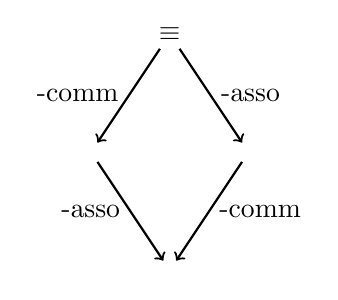
\begin{tikzpicture}[g/.style={outer sep=3pt, inner sep=0pt,minimum width=4pt},e/.style={thick,->}]
		\node[g] (ILL) at (0,0)			{$\LP \equiv \ILL$};
		\node[g] (LC)	at (-1, -1.5)		{$\LC$};
		\node[g] (NL)	at (0, -3)		{$\NL$};
		\node[g] (NLP) at (1, -1.5)		{$\NLP$};
		
		\draw[e] (ILL) -- (LC) node[midway,left]{-comm};
		\draw[e] (LC) -- (NL) node[midway,left]{-asso};
		\draw[e] (ILL) -- (NLP) node[midway,right]{-asso};
		\draw[e] (NLP) -- (NL) node[midway,right]{-comm};
		\
	\end{tikzpicture}
	\label{figure:substructural_logics}
	\caption{$\logic{(N)L(P)}$: $\ILL$ and substructural friends.}
\end{figure}


%\paragraph{Proof nets}
%\todo{}

\section{Restoring Control}
With every step we have taken further into substructuraland, we have been paying a price in expressivity; it is now time for us to acknowledge the accumulated bill.
Dropping \Contraction{} and \Weakening{} made us resource conscious, but theorems of $\IL$ that required resource duplication or erasure became underivable.
Dropping \Exchange{} forced us to pay attention to the order of assumptions, but costed us access to theorems that required permutation to derive.
Substituting the structural comma $\_,\_$ with the non-associative $(\_\sbind\_)$ casted our sequences to trees, this time at the expense of theorems that required rebracketing.
Woe is us -- is there even anything left we can derive?

Perhaps this is painting an overly dramatic picture, considering that none of this is necessarily bad.
From an epistemic perspective, the less structural equivalences we take for granted, the better our mental grasp of structural difference becomes.
In the best case, if it just so happens that the kind of structures we want to investigate overlaps \textit{fully} with the kind of structures our logic can explicitly reason about, the distinction between theorem and non-theorem becomes a refinement rather than a loss of expressivity.
From a more pragmatic perspective, more structural constraints means easier proof search, and less theorems means faster exhaustion of possibilities.
To make the scale of the combinatorics tangible, reflect for a second on this.
A single judgement of $n$ hypotheses in $\NL$ is but one of the Catalan number of bracketings $C(n)$ it would be syntactically undistinguishable from in $\LC$, each one of which in turn is but one of the factorially many permutations $n!$ it would be equivalent to in $\LP$.\footnote{Boom.}
The point to take home is that proof search becomes decidedly easier in the absence of syntactic equivalences, so perhaps a double-edged sword would have made for a better analogy than a bill.

The defeatist attitude here would be to just accept the trade-off between expressivity and complexity, weep for the theorems forever lost, take our victory and walk away.
The problem lies however in the common occasion where the structure of objects under scrutiny overlaps only \textit{partially} with a specific substructural flavor, modulo some exceptional but real cases that require added expressivity.
In such a scenario, taking a step up in the hierarchy would cause an undesirable combinatorial explosion, whereas staying put would sacrifice our ability to argue about these exceptional cases. 
By contrast, the maximalist attitude makes no concessions and seeks both for the cake to be full and the dog to be fed.%
\footnote{Direct translation of a silly but fitting greek aphorism. Cake is bad for dogs.}
What if there was a way to keep our logic computationally tractable but with temporary and on-demand access to normally excluded reasoning tools?

The answer comes in the form of unary \textit{modalities}, type-forming operators lent from modal logics, that allow navigation between logics of different structural properties.
Unary modalities hold a key role in the presentation of full linear logic; there, a single operator $!$ (called \textit{bang}) would allow an embedding of intuitionistic (non-linear) propositions into the linear regime, essentially acting as a licensor of \Contraction{} and \Weakening{}.
In our case, we will make do with two modalities from temporal logic, the diamond $\diamond$ and the box $\Box$, that form a resiudal pair satisfying the accessibility relations:
\begin{center}
\begin{tabularx}{0.5\textwidth}{@{}ccc@{}}
	$ \smallprop{A} \vdash \Box\diamond \smallprop{A}$ & and & $\diamond\Box \smallprop{A} \vdash \smallprop{A}$
\end{tabularx}
\end{center}

\begin{figure}
	\centering
	\begin{tabularx}{0.9875\textwidth}{@{}CC@{}}
		$\infer[\Box E]{\bracket{\Gamma} \vdash \boxelim{\term{s}}: \prop{A}}{
			\Gamma \vdash \term{s}: \Box\prop{A}
		}$
		&
		$\infer[\Box I]{\Gamma \vdash \boxintro{\term{s}}:\Box\prop{A}}{
			\bracket{\Gamma} \vdash \term{s}:\prop{A}
		}$
		\\[2em]
		$\infer[\diamond E]{\Gamma\ctx{\Delta} \vdash \cterm{case \term{\diaelim t} of \term{x_i} in \term{s}}: \prop{B}}{
			\Gamma\ctx{\bracket{\term{x_i}:\prop{A}}}\vdash\term{s}:\prop{B}
			&
			\Delta \vdash \term{t}:\diamond\prop{A}
		}
		$
		&
		$\infer[\diamond I]{\bracket{\Gamma} \vdash \diaintro{\term{s}}: \diamond \prop{A}}{
			\Gamma \vdash \term{s}:\prop{A}
		}$
	\end{tabularx}
	\caption{Logical rules of modal inference.}
	\label{figure:modal_logical}
\end{figure}

The logical manipulation of these modalities is handled by corresponding elimination and introduction rules, presented in Figure~\ref{figure:modal_logical}.
The presentation is intentionally detached from a specific subtructural strand -- modalities are plug-and-play to any member of the $\logic{(N)L(P)}$ family.
Their incorporation adds a new kind of structure to the ones provided by the underlying logic, altering judgements accordingly:
\[
	\Gamma, \Delta, \Theta ::= \dots \ | \ \bracket{\Gamma}
\]
Structures under angular brackets behave differently to the rest; they act as an impenetrable barrier that permits or hinders the introduction or elimination of modal connectives in a judgement.
The box elimination rule $\Box E$ grants us the option of removing a logical box from the succedent of the premise (as long as it is its main connective), but encloses the premises in angular brackets in the process.
Its introduction counterpart $\Box I$ does the exact opposite: it frees a judgement's assumptions from their brackets, but puts the succedent proposition under the scope of a box.
The diamond behaves just the other way around.
Its introduction rule $\diamond I$ is straightforward: it offers the possibility of putting the succedent under the scope of a diamond, in exchange wrapping the antecedents with brackets.
The elimination rule $\diamond E$ is more of a problem child, behaving akin to a unary product.
Without locality restrictions, it inspects a proof of $\smallprop{B}$, the assumptions of which contain a substructure $\bracket{\smallprop{A}}$ within context $\Gamma{\ctx{\_}}$, and allows the post-hoc substitution of the hypothesis together with its brackets by a structure $\Delta$, if from it one can derive $\diamond \smallprop{A}$.

Rules are adorned with term rewrite instructions in the propositions-as-types style~\cite{wansing2002sequent}.
The mnemonic is now two-dimensional: upward triangles denote introduction and downward ones elimination, whereas black triangles are for the box, white ones for the diamond.
Term constructions for the single-premise rules are uncomplicated: each type operation just leaves the corresponding term footprint.
This is not the case for the $\diamond E$ rule, which requires some attention:
the structural substitution of $\bracket{\smallprop{A}}$ for $\Delta$ necessitates a case construct that calls for a term substitution of the variable $\smallterm{x_i}$ for $\diaelim\smallterm{t}$.

\paragraph{Proof \& Term Reductions}
The normalization routines hold as usual

\begin{figure}
	\centering
	\begin{subfigure}{1\textwidth}
		\begin{tabularx}{0.95\textwidth}{@{}ccc@{}}
%		$\infer[\Box E]{\bracket{\Gamma} \vdash \prop{A}}{
%			\infer[\Box I]{\Gamma \vdash \Box \prop{A}}{
%				\infer*[s]{\bracket{\Gamma} \vdash  \prop{A}}{}
%			}
%		}
%		$
%		&
%		\raisebox{10pt}{$\implies$}
%		&
%		$\infer*[s]{\bracket{\Gamma} \vdash \prop{A}}{}
%		$\\[2em]
		$\infer[\diamond E]{\Delta \vdash \diamond\prop{A}}{
			\infer[\diamond I]{\bracket{\prop{A}}\vdash \diamond A}{
				\infer[Ax]{\prop{A} \vdash \prop{A}}{}
			}
			&
			\infer*[s]{\Delta \vdash \diamond\prop{A}}{}
		}$
		&
		\raisebox{20pt}{$\implies$}
		&
		$\infer*[s]{\Delta \vdash \diamond \prop{A}}{}
		$
		\end{tabularx}
	\label{subfigure:123}
	\caption{a}
	\end{subfigure}\\[2em]
	\begin{subfigure}{1\textwidth}
		\begin{tabularx}{0.95\textwidth}{@{}ccc@{}}
%		$\infer[\Box I]{\Gamma \vdash \Box\prop{A}}{
%			\infer[\Box E]{\bracket{\Gamma} \vdash \prop{A}}{
%				\infer*[s]{\Gamma \vdash  \Box\prop{A}}{}
%			}
%		}
%		$
%		&
%		\raisebox{10pt}{$\implies$}
%		&
%		$\infer*[s]{\Gamma \vdash \Box\prop{A}}{}
%		$\\[2em]
		$\infer[\diamond E]{\Gamma\ctx{\bracket{\Delta}} \vdash \prop{B}}{
			\infer*[s]{\Gamma\ctx{\bracket{\prop{A}}} \vdash \prop{B}}{\infer[Ax]{\prop{A} \vdash \prop{A}}{}}
			&
			\infer[\diamond I]{\bracket{\Delta} \vdash \diamond\prop{A}}{
				\infer*[t]{\Delta \vdash \prop{A}}{}
			}
		}
		$
		&
		\raisebox{20pt}{$\implies$}
		&
		$\infer*[s]{\Gamma\ctx{\bracket{\Delta}} \vdash \prop{B}}{
			\infer*[t]{\Delta \vdash \prop{A}}{}
		}
		$
		\end{tabularx}
	\label{subfigure:123}
	\caption{b}
	\end{subfigure}
	\caption{Proof reductions for unary modalities.}
	\label{figure:modal_proof_reductions}
\end{figure}

%, except the latter is now marked with a decoration $\diaelim$.
%This means that the term decoration does not take scope at the outermost layer of term $\smallterm{s}$, but rather nested arbitrarily deeply within it, unlike its better behaved friends.

%is mirrored by a retroactively applied term substitution of the variable $\smallterm{x_i}$ for $\smallterm{t}$, except the latter is now marked with a decoration $\diaelim$ -- this means that the term decoration does not take scope at the outermost layer of term $\smallterm{s}$, but rather nested arbitrarily deeply within it, unlike its better behaved friends.
%Note that here we are breaking our own rules on best practices and using the meta-syntax notation of term substitution; a stricter formulation of the term rewrite would instead be:
%\[
%\]
%We will indulge in the convenience of the substitution version, which makes $\beta$/$\eta$ reductions easier to notice and perform.
%The consequence is that we are conflating multiple terms into a single representation, implicitly establishing a syntactic equivalence on proofs that claims that the exact position of a $\diamond E$ rule is \textit{semantically irrelevant} so long as the same variable $\smallterm{x_i}$ is substituted by the same term $\smallterm{\diaelim t}$.
%

\section{The Linguistic Perspective}

\nocite{sorensen2006lectures}
\nocite{martin1982constructive}

\bibliographystyle{abbrvnat}
\bibliography{bibliography}


